\section{System Implementation Details}
\label{sec:sembloggingsystem}

Based on the process described above, the system is divided between its local part and its remote part, as shown in Figure \ref{fig:semblogsystem}. The local part handles local \emph{private} data, while the remote one handles online \emph{public} data. 
\begin{figure}[htb]
  \begin{center}
    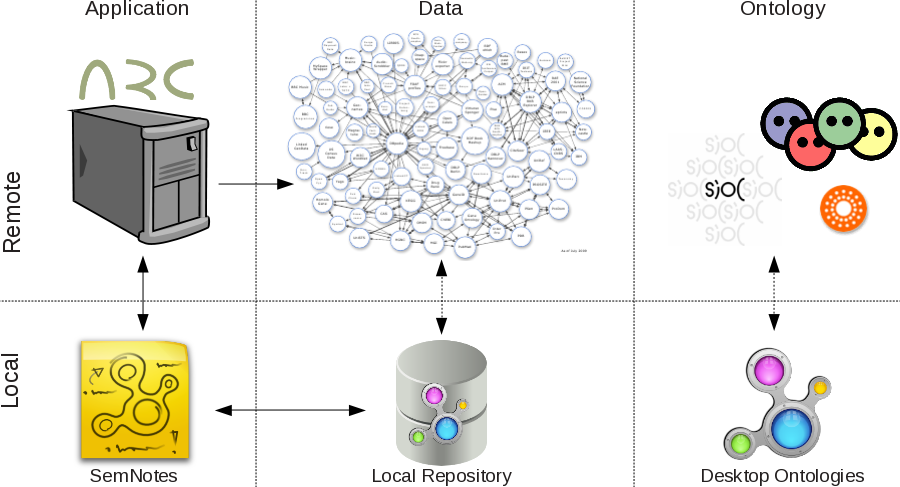
\includegraphics[width=0.8\linewidth]{chapters/core/img/system}
    \caption{Overview of the semantic publishing system.}
    \label{fig:semblogsystem}
  \end{center}
\end{figure}
The separation between them extends over three layers: ontology, data and application.
On the \emph{ontology} layer, the NEPOMUK desktop ontologies are used locally, while popular Web vocabularies are used on the server-side. These ontologies are used to describe the \emph{data} exchanged between the applications. Desktop data is stored in the local NEPOMUK repository, while Web data is distributed. Finally, on the \emph{application} layer, the local component is an extension to SemNotes that provides publishing functionality for notes, and the remote component is a server that hosts and publishes online the notes received.

The first step of the process --- transformation --- is executed on the local side, by an extension of the SemNotes application. Then, the publication step is done by the server, which receives information from the desktop and publishes the note, as we will describe next. The two application components, the communication between them, and the data translation process are described in detail below.

\subsection{Ontologies}

Although both the Semantic Desktop and the Semantic Web use the same representation languages, i.e. RDF(S)/OWL, they use different vocabularies to describe their data. This vocabulary gap makes data integration difficult.

The NEPOMUK project defines a set of desktop ontologies to describe its data.
SemNotes uses these ontologies to represents personal notes as instances of \verb|pimo:Note| and are linked to the \verb|pimo:Thing|s they mention by the relation \verb|pimo:isRelated|. 

When a desktop resource is found to represent the same real world entity as a Web resource, the relation is stored on the desktop as \verb|pimo:hasOtherRepresentation|. This property is recommended by the PIMO specification as desktop equivalent to the \verb|owl:sameAs| relation, although without the formal semantics that the latter provides. We also use the property \verb|pimo:hasOtherRepresentation| to store the remote URL of a note when it is published. If the note changes on the desktop after publication, the property is replaced with \verb|pimo:hasDeprecatedRepresentation|.

While well-suited to represent desktop information, these ontologies are not used, so far, on the Web. However, numerous vocabularies have emerged for describing semantic data published online. Such ontologies have now been widely adopted and are recommended as best practices when publishing data on the Web \cite{Bizer2007}. 

Consequently, while representing similar objects, the two sets of vocabularies must be aligned so that on the one hand, desktop information can be moved to the Web and understood by usual Semantic Web applications that rely on the aforementioned vocabularies, and on the other hand, Web information could be understood and imported by Semantic Desktop applications. In order to enable interoperability between the desktop and the Web, we defined mappings between the sets of ontologies. The mappings create appropriate subclasses or subproperties of the relevant concepts from the chosen vocabularies.

SIOC is probably the most widely used vocabulary for interlinking social media within the Web of Data.
There are already many tools for creating and using SIOC data \cite{Bojars2008}.
This is why we chose to represent the \verb|pimo:Note|s as \verb|sioc:Post|s when they are published online with our system. The rest of the desktop resources are also transformed into concepts from the vocabularies listed above (see Table \ref{tab:classmappings}), the mappings being published at \url{http://rdfs.org/sioc/nepomuk}.
\begin{table}[htb]
\centering
\ra{1.3}
\begin{tabular}{@{}rcl@{}}
\toprule
Class && Subclass of \\ 
\midrule

\verb|pimo:Note| && \verb|sioc:Post| \\

\verb|nao:Tag| && \verb|sioct:Tag| \\

\verb|pimo:Person| && \verb|foaf:Person| \\

\verb|pimo:Project| && \verb|doap:Project| \\

\verb|pimo:Event| && \verb|ical:Vevent| \\

\bottomrule
\end{tabular}
\caption{Sample of the mapping between classes.}
\label{tab:classmappings}
\end{table}
The note's properties, like title, creation and last modification time, are translated to the appropriate Dublin Core properties: \verb|dcterm:created|, \verb|dcterms:modified| and \verb|dcterms:title|. The tags associated locally with the notes are transformed into \verb|sioct:Tag|s associated with the published post using the \verb|sioc:topic| property. Table \ref{tab:propmappings} lists the proposed mappings for properties\footnote{Although \texttt{nao:lastModified} and \texttt{dcterms:modified} do not have the same semantics, defining subproperty relations between them is acceptable.}.

\begin{table}[htb]
\centering
\ra{1.3}
\begin{tabular}{@{}rcl@{}}
\toprule
Property && Subproperty of \\ 
\midrule

\verb|nao:prefLabel| && \verb|rdfs:label| \\

\verb|nao:created| && \verb|dcterms:created| \\

\verb|nao:lastModified| && \verb|dcterms:modified| \\

\verb|nao:hasTag| && \verb|sioc:topic| \\

\verb|pimo:isRelated| && \verb|sioc:related_to| \\

\bottomrule
\end{tabular}
\caption{Sample of the mapping between properties.}
\label{tab:propmappings}
\end{table}


\subsection{Server Schema}

In order to publish the resources with a consistent URI scheme, we defined patterns for naming the objects published from the desktop on the Web. In the schema definition, we apply several Linked Data patterns described in \cite{Dodds2010LDPBook}: 
\begin{itemize} 
 \item patterned URIs --- for all the entities, to make them more human readable; 
 \item proxy URIs --- for the server URIs, to group multiple Web aliases;
 \item equivalence links --- for the resources related to the notes, to unify various sources; 
 \item natural keys --- in the tag URIs. 
\end{itemize}

For each note the server generates a new unique identifier \verb|id| which is used to create the note's URI in the form: \verb|http://notes.server/note/id|.

According to the proxy URIs identifier creation pattern, we generate new URIs for the resources related to the notes. This ensures that the publishing process is consistent and avoids having to choose among several Web aliases a resource could have. Like the notes, each resource has a unique identifier on the server, which is used to create the resource URI according to the following format: \verb|http://notes.server/resource/id|. Resources are shared by all the notes that link to them, which increases the interlinking and the consistency of the data. For each resource, the server keeps internally a list of Web aliases using \verb|owl:sameAs| links.

Tags are considered a particular type of resources, and are also shared on the server. The specific format for the URI: \verb|http://notes.server/tag/label|, differentiates them from regular resources. The label of the tag acts as a unique identifier, and is case sensitive. They are created on the fly, and are persisted when they are used for the first time.


\subsection{Transformation of the Notes for Sharing}

The first step of the process consists of preparing the note for publishing. In this phase all the relevant information about the note is included in the content, specifically the title, creation and last modification time, the tags and the referenced resources. This transformation is necessary, so that less information, specifically only the HTML content of the note is sent to the server, and not the entire RDF graph describing the note. Although the content is already stored as HTML, to include all the metadata about the note, it has to be enriched with RDFa before being posted to the server.

The preparation step is done on the desktop side, by the added extension to SemNotes. 
To include the referenced resources in RDFa, we need to know their server URIs. Therefore the application needs to communicate with the server to retrieve several URIs: 
\begin{itemize}
 \item the URI for the new note to be published, and 
 \item the server URI for each resource referenced by the note. 
\end{itemize}

In case the note has already been published, the user can overwrite the old post (on the Web) or create a new one. Depending on this choice, a new URI is requested from the server, or the existing one is used (that was saved in the local repository when the note was previously published). 

The referenced resources are shared by all the published notes, therefore the server must create the URI for a resource only if it has not been created before. To decide whether a local resource already has a server URI created, the list of Web aliases found for it on the desktop in the second prerequisite step of the process, is sent to the server (see JSON data in Listing \ref{lst:messagetoserver}). If a resource with a matching type and an overlapping list of aliases exists, the server reuses it, otherwise it creates a new one and saves the information about it in its own RDF repository. On the server, the URI aliases are saved as \verb|owl:sameAs| as it is customary for Linked Data. The server URIs for the note and the resources are also stored on the desktop for reuse, as \verb|pimo:hasOtherRepresentation|.
\lstset{
	caption={JSON formatted message sent to the server.}, 
	label=lst:messagetoserver,
	language=js
}
\setlength\parindent{0in}
\begin{minipage}[t]{\linewidth}
\begin{lstlisting}
{
   "id" : "",
   "resources": [
   {
      "id": "nepomuk:/res/bfcdcd1a-4898-492f-940b-4cc4c67799a7",
      "type": "mo:MusicArtist",
      "uris": [
         "http://dbpedia.org/resource/Scorpions_(band)",
         "http://musicbrainz.org/artist/c3cceeed-3332-4cf0-8c4c-bbde425147b6"
      ]
   }
   ]
}
\end{lstlisting}
\end{minipage}
\setlength\parindent{0.21in}

\lstset{
	caption={Server reply with the server URIs for the resource aliases sent.}, 
	label=lst:serverreply,
	language=js
}
\setlength\parindent{0in}
\begin{minipage}[t]{\linewidth}
\begin{lstlisting}
{
   "note":{
      "uri":"http://notes.server/note/4baccab834e20",
      "resources":[
         {
            "local":"nepomuk:/res/bfcdcd1a-4898-492f-940b-4cc4c67799a7",
            "uri":"http://notes.server/resource/4bacca84ca8bb"
         }
      ]
   }
}
\end{lstlisting}
\end{minipage}
\setlength\parindent{0.21in}

In the case when no Web aliases are found for a desktop resource that is related to a note, and thus the list of aliases sent to the server is empty, a new resource is created on the server with the specified type, but without any information attached to it. The server URI is saved on the desktop as \verb|pimo:hasOtherRepresentation| of the resource, and will be available for reuse when other notes related to the same object are published by the same user. However, this resource will not be shared between notes published by different users. If at a later stage a Web alias is found for the desktop resource, it will be added to the resource already created on the server, thus enabling it to be linked to by multiple users.

The communication between SemNotes and the server is done with a single REST call, in order to minimise network delays. The reply contains the newly created URI for the note, if one was required, as well as a list of server URIs for the resources (see JSON data in Listing \ref{lst:serverreply}). The communication between the desktop side and the server is shown in Figure \ref{fig:semblogsequencediag}. 

Using the information received from the server, the note content is enriched with RDFa. The metadata about the note, like type, creation and last modification times and the tags, is added in \verb|meta| tags in the \verb|head| of the HTML page. RDFa is added to the \verb|title| tag and in the \verb|body|, to the links. Listing \ref{lst:rdfa} shows the content of a note prepared for publishing.

\begin{figure}[htb]
  \begin{center}
    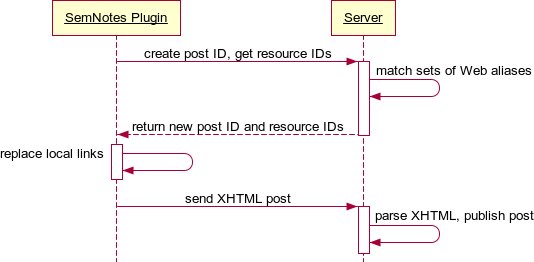
\includegraphics[width=0.85\linewidth]{chapters/core/img/sequencediagram}
    \caption{Sequence diagram for the communication with the server.}
    \label{fig:semblogsequencediag}
  \end{center}
\end{figure}

\lstset{
	caption={RDFa-annotated XHTML content of note.}, 
	label=lst:rdfa,
	language=htmlrdfa
}
\setlength\parindent{0in}
\begin{minipage}[t]{\linewidth}
\begin{lstlisting}
<!DOCTYPE html PUBLIC '-//W3C//DTD XHTML RDFa 1.0//EN' 
                      'http://www.w3.org/MarkUp/DTD/xhtml-rdfa-1.dtd'>
<html about="http://notes.server/note/4baccab834e20">
    <head>
        <meta content="sioc:Post" property="rdf:type"/>
        <meta rel="sioc:topic" href="http://notes.server/tag/concert"/>
        <title property="dc:title">concert sunday</title>
    </head>
    <body>
        <a rel="sioc:is_related"
             href="http://notes.server/resource/4bacca84ca8bb">scorpions</a> concert on sunday was great ...
    </body>
</html>
\end{lstlisting}
\end{minipage}
\setlength\parindent{0.21in}


\subsection{Publication Step}

After the preparation step, which takes place on the desktop side, the RDFa enriched content is sent to the server via another REST call. The publication step of the process only handles public data. When the content is received it is parsed and the server extracts the contained RDF triples and stores them in its repository. The content (as it is received) is also stored.

The server implementation uses ARC2\footnote{\url{http://arc.semsol.org}}, as it provides out of the box RDFa parsing and an RDF repository. It is easily deployable due its minimal setup requirements (a PHP enabled Web server and a MySQL database), thus making our system easily deployable as well.

All server URIs are dereferenceable, as required by the Linked Data principles. For notes, the URI redirects to the RDFa annotated HTML page containing the note itself (as shown in Figure \ref{fig:views} (i)), the URI of the note being the URL of this page. For the linked resources, the URI is also dereferenceable and provides RDFa information about itself, linking to the known existing Web aliases of the same resource. The description also includes a list of backlinks to all the notes that reference the resource (see Figure \ref{fig:views} (ii)). The page for a tag will contain backlinks to all the notes tagged with it.

The RDFa annotated page for the note is generated on the user's desktop by the SemNotes plugin, as we have seen in the previous step, while the page describing each resource and tag is generated on the fly, by the server, when the URI is requested.

\begin{figure}[tb]
\begin{minipage}[b]{0.49\linewidth}
\begin{flushleft}
    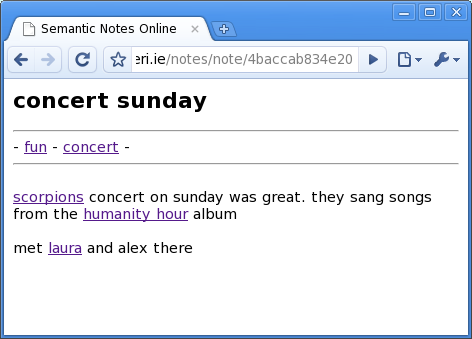
\includegraphics[width=0.97\linewidth]{chapters/core/img/noteview}
\end{flushleft}
\end{minipage}
\begin{minipage}[b]{0.49\linewidth}
\begin{flushright}
    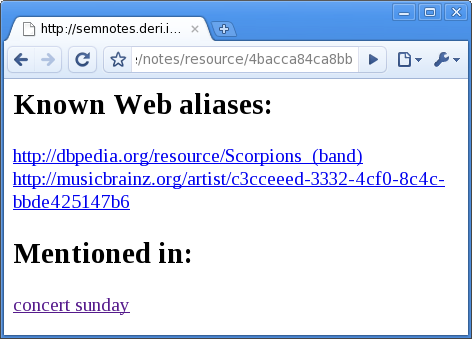
\includegraphics[width=0.97\linewidth]{chapters/core/img/resourceview}
\end{flushright}
\end{minipage}
\caption{Online view of a note (i) and a resource (ii).}
\label{fig:views}
\end{figure}
